\documentclass[11pt,a4paper]{ctexart}

% ============================ 宏包 ============================
\usepackage{amsmath,amssymb,amsthm,mathtools}
\usepackage{geometry}
\geometry{left=2.35cm,right=2.35cm,top=2.5cm,bottom=2.4cm}
\usepackage{graphicx}
\usepackage{float}
\usepackage{caption}
\usepackage{xcolor}
\usepackage{enumitem}
\usepackage{booktabs}
\usepackage{array}
\usepackage{tikz}
\usetikzlibrary{arrows.meta,positioning,decorations.pathreplacing,calc}
\usepackage{fancyhdr}
\usepackage{tcolorbox}
\tcbuselibrary{skins,breakable}
\usepackage{titlesec}
\usepackage{needspace}
\usepackage{hyperref}
\hypersetup{colorlinks=true,linkcolor=teal!60!black,
            urlcolor=teal!60!black,citecolor=teal!60!black}

% ============================ 字体与格式 ============================
\setCJKmainfont{SimSun}[BoldFont=SimHei,ItalicFont=KaiTi]
\setCJKsansfont{Microsoft YaHei}
\setCJKfamilyfont{kai}{KaiTi}
\providecommand{\kaishu}{}
\renewcommand{\kaishu}{\CJKfamily{kai}}

\definecolor{mainc}{RGB}{31,78,121}
\definecolor{upc}{RGB}{192,57,43}
\definecolor{downc}{RGB}{30,132,73}
\definecolor{orangec}{RGB}{230,126,34}
\definecolor{purplec}{RGB}{108,52,131}
\definecolor{lightbg}{RGB}{246,248,251}

\captionsetup[figure]{font=small,labelfont={bf,color=mainc},
                      labelsep=quad,textfont=small}
\captionsetup[table]{font=small,labelfont={bf}}

\titleformat{\section}{\Large\bfseries\color{mainc}}{\thesection}{0.8em}{}
\titleformat{\subsection}{\large\bfseries\color{mainc}}{\thesubsection}{0.7em}{}
\titleformat{\subsubsection}{\normalsize\bfseries}{\thesubsubsection}{0.6em}{}
\titlespacing*{\section}{0pt}{1.6em}{0.8em}

\setlist[itemize]{leftmargin=1.6em,itemsep=2pt,topsep=4pt}
\setlist[enumerate]{leftmargin=1.9em,itemsep=2pt,topsep=4pt}

\linespread{1.28}

% 定理环境
\theoremstyle{definition}
\newtheorem{theorem}{定理}[section]
\newtheorem{lemma}[theorem]{引理}
\newtheorem{corollary}[theorem]{推论}
\newtheorem{example}[theorem]{例}
\newtheorem{proposition}[theorem]{命题}
\newtheorem{definition}[theorem]{定义}

\theoremstyle{remark}
\newtheorem*{remark}{注}
\newtheorem*{proofidea}{思路}
\newtheorem*{counter}{反例}

\renewcommand{\proofname}{\bfseries 证明}
\renewcommand\qedsymbol{$\blacksquare$}

% 常用记号
\newcommand{\R}{\mathbb{R}}
\newcommand{\N}{\mathbb{N}}
\newcommand{\Q}{\mathbb{Q}}
\newcommand{\eps}{\varepsilon}
\newcommand{\abs}[1]{\left\lvert #1 \right\rvert}
\newcommand{\norm}[1]{\left\lVert #1 \right\rVert}
\newcommand{\limn}{\lim_{n\to\infty}}
\newcommand{\dd}{\,\mathrm{d}}
\newcommand{\U}{\mathcal{U}}
\newcommand{\xra}[1]{\xrightarrow{#1}}

% 自定义盒子
\newtcolorbox{keybox}[1][]{
  colback=lightbg, colframe=mainc, boxrule=0.7pt, arc=2pt,
  left=7pt,right=7pt,top=5pt,bottom=5pt,
  fonttitle=\bfseries\color{white}, coltitle=white,
  colbacktitle=mainc, title={#1},
  breakable, enhanced
}
\newtcolorbox{warnbox}[1][]{
  colback=orangec!6, colframe=orangec!85!black, boxrule=0.7pt, arc=2pt,
  left=7pt,right=7pt,top=5pt,bottom=5pt,
  fonttitle=\bfseries\color{white}, coltitle=white,
  colbacktitle=orangec!85!black, title={#1},
  breakable, enhanced
}
\newtcolorbox{tipbox}[1][]{
  colback=downc!6, colframe=downc!80!black, boxrule=0.7pt, arc=2pt,
  left=7pt,right=7pt,top=5pt,bottom=5pt,
  fonttitle=\bfseries\color{white}, coltitle=white,
  colbacktitle=downc!80!black, title={#1},
  breakable, enhanced
}

\pagestyle{fancy}
\fancyhf{}
\fancyhead[L]{\small\color{mainc} 数学分析专题笔记}
\fancyhead[R]{\small\color{mainc} $\varepsilon$\text{-}$\delta$ 语言}
\fancyfoot[C]{\small\thepage}
\renewcommand{\headrulewidth}{0.4pt}
\renewcommand{\headrule}{\hbox to\headwidth{\color{mainc}\leaders\hrule height \headrulewidth\hfill}}

\begin{document}

% ============================ 封面 ============================
\begin{titlepage}
\centering
\vspace*{2.4cm}

{\color{mainc}\rule{\linewidth}{1.6pt}}\\[0.9cm]

{\Huge\bfseries $\boldsymbol{\varepsilon}$-$\boldsymbol{\delta}$ 语言完全笔记\par}
\vspace{0.5cm}
{\LARGE\bfseries 从数列极限到一致连续\par}
\vspace{0.35cm}
{\large 定义 · 否定形式 · 数轴图像 · 全部证明 · 反例\par}

\vspace{0.6cm}
{\color{mainc}\rule{\linewidth}{1.6pt}}

\vspace{2.4cm}

{\large\kaishu
\begin{tabular}{rl}
\textbf{核心内容} & $\varepsilon$\text{-}$N$（数列）· $\varepsilon$\text{-}$\delta$（函数）· $\varepsilon$\text{-}$M$（无穷远）\\[4pt]
                & 连续 · 一致连续 · Heine 定理 · Cauchy 准则\\[4pt]
\textbf{方法}   & 量词否定 · “先估计再取 $\delta$” · “放大—控制”证明模板\\[4pt]
\textbf{图像}   & 8 幅数轴/带状示意图（$\varepsilon$ 带、$\delta$ 邻域）\\[4pt]
\textbf{重点}   & 一致连续与连续的区别：$\delta$ 能否与 $x_0$ 无关\\[4pt]
\end{tabular}}

\vfill

{\large 共 \textbf{26} 条定义与定理，\textbf{28} 个完整证明与反例}

\vspace{1.0cm}
{\color{mainc}\rule{0.45\linewidth}{0.8pt}}
\end{titlepage}

\tableofcontents
\newpage

% ============================ 第 0 章 ============================
\section{为什么需要 $\varepsilon$\text{-}$\delta$ 语言}

\subsection{从“无限接近”到“可以任意小”}

初学微积分时，我们说 $a_n$ “趋于”$A$，直觉是“$a_n$ 越来越靠近 $A$、而且要多近有多近”。
这句话的问题在于它\emph{不可证伪}：怎样才算“要多近有多近”？不同的人可以有不同的理解。

$\varepsilon$\text{-}$\delta$ 语言做的事情是：\textbf{把“无限接近”翻译成有限的不等式}。
其核心思想是\emph{挑战—应答}（challenge--response）模型：

\begin{keybox}[挑战—应答模型]
\begin{itemize}
  \item \textbf{挑战方}：给出任意一个允许误差 $\eps>0$（无论多小）。
  \item \textbf{应答方}：必须给出一个相应的门槛（$N$ 或 $\delta$ 或 $M$）。
  \item \textbf{检验}：一旦越过这个门槛，待比较的量与目标值的差就小于 $\eps$。
  \item \textbf{定义成立}：应答方对\emph{每一个}挑战都能给出应答，且应答\emph{可以依赖}挑战。
\end{itemize}
“$\forall\eps>0\ \exists\delta>0$” 读作“对任取的 $\eps$，我们都能找到 $\delta$”——
\textbf{$\delta$ 是 $\varepsilon$ 的函数}，这正是整个理论的关键。
\end{keybox}

\subsection{三种形式一览}

本书讨论三种同构的形式，它们只差“往哪边收缩”：

\begin{figure}[H]
  \centering
  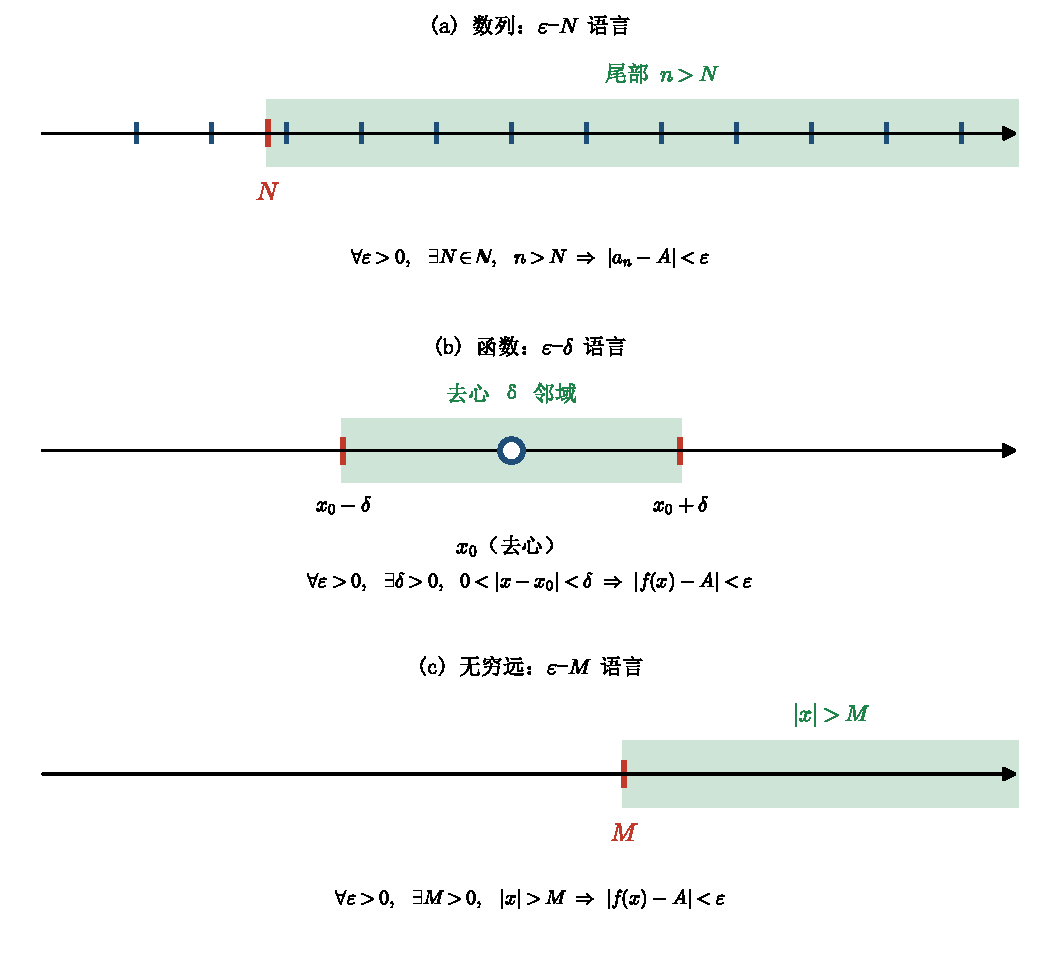
\includegraphics[width=0.99\textwidth]{figures/fig8_three_langs.pdf}
  \caption{三种语言的数轴图像。(a) 数列：$N$ 之后的\emph{尾巴}必须落在 $A$ 的 $\eps$ 带内；
           (b) 函数：$x_0$ 的\emph{去心 $\delta$ 邻域}必须被映到 $A$ 的 $\eps$ 带内（空心圆表示 $x_0$ 本身可以不管）；
           (c) 无穷远：$\abs{x}>M$ 的\emph{远端}必须落在带内。三者的逻辑骨架完全一致。}
  \label{fig:three}
\end{figure}

\begin{table}[H]
\centering
\caption{三种 $\eps$-语言对照（$A$ 为极限值）}
\renewcommand{\arraystretch}{1.55}
\small
\begin{tabular}{@{}llll@{}}
\toprule
\textbf{对象} & \textbf{记号} & \textbf{定义} & \textbf{门槛} \\
\midrule
数列 & $a_n\to A$ & $\forall\eps>0\ \exists N\ \forall n>N:\ \abs{a_n-A}<\eps$
     & $N\in\N$ \\
函数 & $f(x)\to A\ (x\to x_0)$ &
     $\forall\eps>0\ \exists\delta>0\ \forall x:\ 0<\abs{x-x_0}<\delta\Rightarrow\abs{f(x)-A}<\eps$
     & $\delta>0$ \\
无穷远 & $f(x)\to A\ (x\to\infty)$ &
     $\forall\eps>0\ \exists M>0\ \forall x:\ \abs{x}>M\Rightarrow\abs{f(x)-A}<\eps$
     & $M>0$ \\
\bottomrule
\end{tabular}
\end{table}

\newpage

% ============================ 第 1 章 ============================
\section{数列极限与 $\varepsilon$\text{-}$N$ 语言}

\subsection{定义}

\begin{definition}[数列极限]\label{def:seq}
设 $\{a_n\}$ 为实数列，$A\in\R$。若
\begin{equation}\label{eq:epsN}
  \forall\eps>0,\quad \exists N\in\N,\quad \forall n>N:\quad \abs{a_n-A}<\eps,
\end{equation}
则称 $\{a_n\}$ \textbf{收敛于} $A$，记作 $\limn a_n=A$ 或 $a_n\to A$。
\end{definition}

\begin{figure}[H]
  \centering
  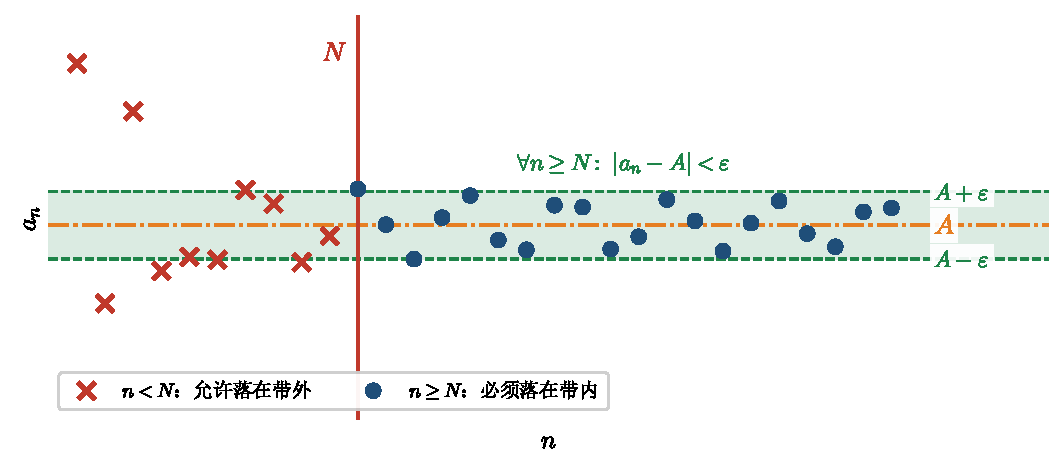
\includegraphics[width=0.95\textwidth]{figures/fig1_epsilon_N.pdf}
  \caption{$\varepsilon$\text{-}$N$ 定义的数轴图像。给定 $\eps$（这里 $\eps=0.28$），
           在 $A$ 上下画出 $\eps$ 带。$N$ 之前（红叉）可以有任意有限多项落在带外；
           $N$ 之后（蓝点）\emph{所有}项都必须落在带内。$\eps$ 变小则 $N$ 变大。}
  \label{fig:epsN}
\end{figure}

\begin{warnbox}[读定义的四个要点]
\begin{enumerate}[label=\arabic*.]
  \item \textbf{$\eps$ 在前，$N$ 在后}：$N$ 可以依赖 $\eps$。
        “$\exists N\ \forall\eps$” 是\emph{完全不同}的（错误的）命题。
  \item \textbf{$\eps>0$ 是严格的}：$\eps=0$ 不允许。$\eps$ 是“允许误差”，必须为正。
  \item \textbf{是“$n>N$”而不是“$n\ge N$”}：两者等价（把 $N$ 换成 $N+1$ 即可），
        但不要在同一证明中混用。
  \item \textbf{前有限项无关紧要}：改变数列的有限多项不影响其敛散性与极限值。
\end{enumerate}
\end{warnbox}

\subsection{否定形式：$\varepsilon$\text{-}$N$ 的取反}

\begin{theorem}[极限不成立]\label{thm:neg-seq}
“$a_n\to A$” 不成立，当且仅当
\begin{equation}\label{eq:neg-epsN}
  \exists\eps_0>0,\quad \forall N\in\N,\quad \exists n>N:\quad \abs{a_n-A}\ge\eps_0 .
\end{equation}
\end{theorem}

\begin{proof}
记命题 $P$ 为 \eqref{eq:epsN}，即
$P:\ \forall\eps>0\ \exists N\ \forall n>N\ Q(n,\eps)$，其中 $Q$ 是“$\abs{a_n-A}<\eps$”。

\textbf{逐层取反}。按规则 $\overline{\forall x\,R}=\exists x\,\overline{R}$ 与
$\overline{\exists x\,R}=\forall x\,\overline{R}$：
\[
  \overline{P}:\quad
  \exists\eps>0\ \ \overline{\exists N\ \forall n>N\ Q}
  \ \equiv\
  \exists\eps>0\ \forall N\ \ \overline{\forall n>N\ Q}
  \ \equiv\
  \exists\eps>0\ \forall N\ \exists n>N\ \overline{Q}.
\]
其中 $\overline{Q}$ 是 $\abs{a_n-A}<\eps$ 的否定，即 $\abs{a_n-A}\ge\eps$。
把哑元 $\eps$ 改名为 $\eps_0$ 即得 \eqref{eq:neg-epsN}。

\textbf{为什么每一层都这么翻}：$\forall N\ \exists n>N\ \abs{a_n-A}\ge\eps_0$ 的意思是
“无论门槛 $N$ 取得多大，我总能在它\emph{之后}再找到一个坏项”。
这正好排除了“最终所有项都进带”这种好局面。

\end{proof}

\begin{keybox}[否定形式的记忆口诀]
\textbf{“存在一个 $\eps_0$，使得无限多项跑到 $\eps_0$ 带外。”}
\par\smallskip
形式上是把“$\forall\eps\ \exists N\ \forall n$”读成“任意误差都能被\emph{尾部}吸收”，
它的反面就是“有某个固定误差，\emph{尾部}永远吸收不掉”——也就是\emph{无穷多个}坏项。
\end{keybox}

\begin{counter}[极限不存在]\label{counter:oscillate}
$a_n=(-1)^n$ 不收敛。
\end{counter}

\begin{proof}
取 $\eps_0=1$。对任意 $N$，令 $n$ 为大于 $N$ 的奇数，则 $a_n=-1$；再令 $m$ 为大于 $N$
的偶数，则 $a_m=1$。若极限 $A$ 存在，则
\[
  \abs{a_n-A}<\eps_0=1\quad\text{且}\quad\abs{a_m-A}<1 .
\]
但 $\abs{a_m-a_n}=2$，与三角不等式 $\abs{a_m-a_n}\le\abs{a_m-A}+\abs{A-a_n}<2$ 矛盾。
因此对任何 $A$ 都无法满足 \eqref{eq:epsN}，特别地取 $n$ 为奇数时
$\abs{a_n-A}\ge1$ 对无穷多个 $n$ 成立，符合 \eqref{eq:neg-epsN}。

\end{proof}

\subsection{基本证明模板}

\begin{keybox}[$\eps$-$N$ 证明的四步模板]
\begin{enumerate}[label=\textbf{步骤 \arabic*.}, leftmargin=4.2em]
  \item \textbf{写出差值并估计}：把 $\abs{a_n-A}$ 变形，找到只依赖 $n$ 的上界，通常是
        $\abs{a_n-A}\le \dfrac{C}{f(n)}$ 型。
  \item \textbf{令上界 $<\eps$ 反解}：由 $\dfrac{C}{f(n)}<\eps$ 解出 $n>f^{-1}(C/\eps)$。
  \item \textbf{取 $N$}：取 $N=\left\lceil f^{-1}(C/\eps)\right\rceil$（取整，保证是自然数）。
  \item \textbf{回代验证}：对 $n>N$ 走一遍，确认 $\abs{a_n-A}<\eps$。
\end{enumerate}
\textbf{注意}：证明中“取 $N=\dots$”这一步，写的是\emph{构造}而非\emph{求解}。
只要能说明该 $N$ 存在即可，不必求出“最小的 $N$”。
\end{keybox}

\begin{example}[基本型]\label{ex:basic}
证明 $\displaystyle\limn\frac{2n+1}{n+3}=2$。
\end{example}

\begin{proof}
\textbf{步骤 1（估计）}：
\[
  \abs{\frac{2n+1}{n+3}-2}
  =\abs{\frac{2n+1-2n-6}{n+3}}
  =\frac{5}{n+3}\ <\ \frac{5}{n},
\]
因为 $n+3>n$。

\textbf{步骤 2（反解）}：要求 $\frac5n<\eps$，即 $n>\frac5\eps$。

\textbf{步骤 3（取 $N$）}：取 $N=\left\lceil\frac{5}{\eps}\right\rceil$。

\textbf{步骤 4（验证）}：当 $n>N\ge\frac5\eps$ 时，
$\frac{5}{n}<\eps$，故 $\abs{\frac{2n+1}{n+3}-2}<\eps$。
由 $\eps>0$ 的任意性，极限为 $2$。

\end{proof}

\begin{example}[含根号，需要有理化]\label{ex:sqrt}
证明 $\displaystyle\limn\bigl(\sqrt{n+1}-\sqrt n\bigr)=0$。
\end{example}

\begin{proof}
\textbf{步骤 1}：分子有理化
\[
  \abs{\sqrt{n+1}-\sqrt n}
  =\frac{(\sqrt{n+1}-\sqrt n)(\sqrt{n+1}+\sqrt n)}{\sqrt{n+1}+\sqrt n}
  =\frac{1}{\sqrt{n+1}+\sqrt n}
  <\frac{1}{2\sqrt n}.
\]
（这里用到 $\sqrt{n+1}>\sqrt n$，故分母 $>2\sqrt n$。）

\textbf{步骤 2--3}：要求 $\frac{1}{2\sqrt n}<\eps$，即 $\sqrt n>\frac{1}{2\eps}$，
即 $n>\frac{1}{4\eps^{2}}$。取
\[
  N=\left\lceil\frac{1}{4\eps^{2}}\right\rceil .
\]
\textbf{步骤 4}：当 $n>N$ 时上述不等式链给出 $\abs{\sqrt{n+1}-\sqrt n}<\eps$。

\end{proof}

\begin{example}[指数型，用单调性]\label{ex:exp-seq}
设 $0<q<1$。证明 $\limn q^{n}=0$。
\end{example}

\begin{proof}
\textbf{步骤 1}：因为 $0<q<1$，可写 $q=\frac{1}{1+h}$，其中 $h=\frac1q-1>0$。
由伯努利不等式（$(1+h)^n\ge 1+nh$）：
\[
  \abs{q^{n}-0}=q^{n}=\frac{1}{(1+h)^{n}}\le\frac{1}{1+nh}<\frac{1}{nh}.
\]
\textbf{步骤 2--3}：要求 $\frac{1}{nh}<\eps$，即 $n>\frac{1}{h\eps}$。取
$N=\left\lceil\frac{1}{h\eps}\right\rceil$。

\textbf{步骤 4}：$n>N$ 时 $q^n<\frac{1}{nh}<\eps$。

\end{proof}

\begin{example}[取对数型]\label{ex:log}
证明 $\displaystyle\limn\frac{\ln n}{n}=0$。
\end{example}

\begin{proof}
\textbf{思路}：用 $\ln n\le n-1$ 太弱，改用 $\ln n\le\sqrt n$（对 $n\ge1$）可以给出 $n^{-1/2}$ 的界。

\textbf{步骤 1}：先验证 $\ln n\le\sqrt n$。令 $\varphi(x)=x-2\ln x$（$x\ge1$），
则 $\varphi(1)=1>0$，$\varphi'(x)=1-\frac2x$，在 $[1,2]$ 上 $\varphi'\le0$、
在 $[2,\infty)$ 上 $\varphi'\ge0$；故 $\varphi$ 在 $x=2$ 处取最小值
$\varphi(2)=2-2\ln2\approx0.614>0$。因此 $\varphi>0$，即 $\ln x<x$，
令 $x=\sqrt n$ 得 $\ln\sqrt n<\sqrt n$，即 $\frac12\ln n<\sqrt n$，从而
\(
  \ln n<2\sqrt n
\)。

\textbf{步骤 2--3}：于是
\[
  0\le\frac{\ln n}{n}<\frac{2\sqrt n}{n}=\frac{2}{\sqrt n}.
\]
要求 $\frac{2}{\sqrt n}<\eps$，即 $n>\frac{4}{\eps^{2}}$。取
$N=\left\lceil\frac{4}{\eps^{2}}\right\rceil$。

\textbf{步骤 4}：$n>N$ 时 $0\le\frac{\ln n}{n}<\eps$，故极限为 $0$。

\end{proof}

\begin{tipbox}[“放大”的艺术]
四个例子的共同点是：\textbf{把复杂的 $\abs{a_n-A}$ 放大成一个形式简单、容易反解的量}。
放大的方向必须让\emph{不等号指向需要的方向}，而且放大后的量必须\textbf{趋于 $0$}。
放得太大（如例~\ref{ex:log} 中直接用 $\ln n<n$ 得 $\frac{\ln n}{n}<1$）就无法反解出 $N$。
\end{tipbox}

\subsection{Cauchy 收敛准则}

\begin{theorem}[Cauchy 准则]\label{thm:cauchy}
实数列 $\{a_n\}$ 收敛 $\iff$ 它是 \textbf{Cauchy 列}，即
\begin{equation}\label{eq:cauchy}
  \forall\eps>0,\quad \exists N\in\N,\quad \forall m,n>N:\quad \abs{a_m-a_n}<\eps .
\end{equation}
\end{theorem}

\begin{figure}[H]
  \centering
  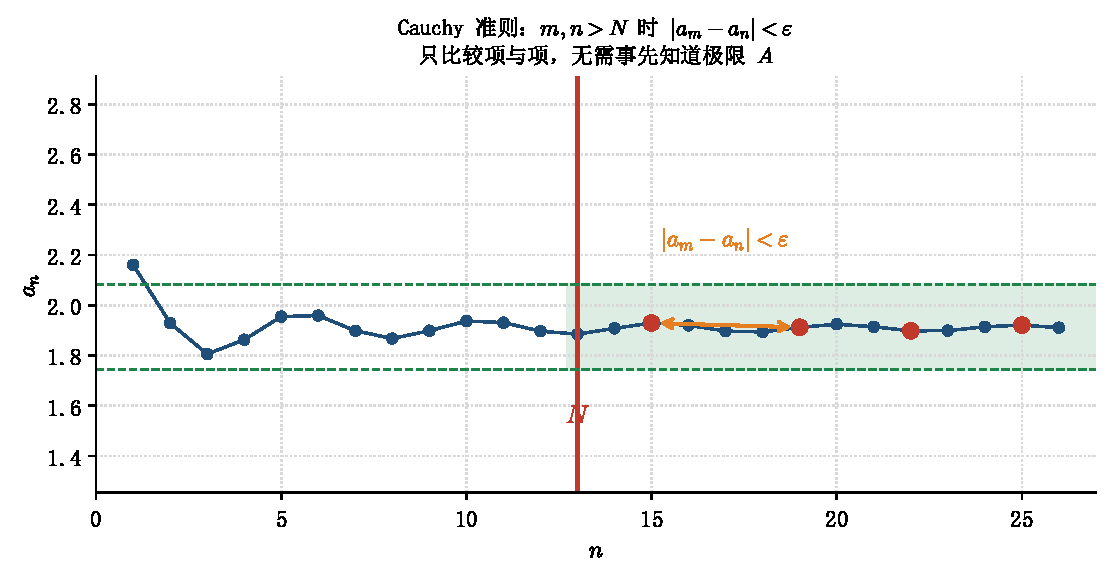
\includegraphics[width=0.86\textwidth]{figures/fig9_cauchy.pdf}
  \caption{Cauchy 准则的图像。$N$ 之后取任意两项 $a_m,a_n$，它们的差都小于 $\eps$。
           与 $\eps$-$N$ 定义的关键差别是：\textbf{不需要事先知道极限值 $A$}，
           只比较项与项。这正是它在构造实数（完备化）时的价值。}
  \label{fig:cauchy}
\end{figure}

\begin{proof}[\bfseries 必要性（$\Rightarrow$）]
设 $a_n\to A$。给定 $\eps>0$，由定义取 $N$ 使 $n>N$ 时 $\abs{a_n-A}<\frac{\eps}{2}$。
则对 $m,n>N$：
\[
  \abs{a_m-a_n}\le\abs{a_m-A}+\abs{A-a_n}<\frac\eps2+\frac\eps2=\eps .
\]
（这里用到了三角不等式，以及“把 $\eps$ 换成 $\eps/2$ 仍然可用”，这是分析中的常用技巧。）

\end{proof}

\begin{proof}[\bfseries 充分性（$\Leftarrow$）]
充分性需要 $\R$ 的完备性。分三步。

\textbf{第 1 步：Cauchy 列有界。}取 $\eps=1$，得 $N_1$ 使 $m,n>N_1$ 时 $\abs{a_m-a_n}<1$。
固定 $n_0=N_1+1$，则对一切 $n>N_1$：
\[
  \abs{a_n}\le\abs{a_n-a_{n_0}}+\abs{a_{n_0}}<1+\abs{a_{n_0}}.
\]
而前 $N_1$ 项只有有限多个数，故有界。于是整个数列有界。

\textbf{第 2 步：取子列。}由波尔查诺—魏尔斯特拉斯定理，有界数列有收敛子列
$a_{n_k}\to A$（$k\to\infty$）。下面证明\emph{整个}数列收敛到同一个 $A$。

\textbf{第 3 步：用 Cauchy 性质把子列的极限传给全体。}给定 $\eps>0$。
由 Cauchy 条件取 $N_2$ 使 $m,n>N_2$ 时 $\abs{a_m-a_n}<\frac\eps2$。
由 $a_{n_k}\to A$ 取 $K$ 使 $k\ge K$ 时 $\abs{a_{n_k}-A}<\frac\eps2$，
并且要求 $n_k>N_2$（因 $n_k\to\infty$，总可做到）。取
$N_0=\max\{N_2,n_K\}$。对任意 $n>N_0$，取一个 $k\ge K$，则 $n_k>N_2$ 且 $n>N_2$，于是
\[
  \abs{a_n-A}\le\abs{a_n-a_{n_k}}+\abs{a_{n_k}-A}<\frac\eps2+\frac\eps2=\eps .
\]
故 $a_n\to A$。

\end{proof}

\begin{remark}
步骤 2 用的 Bolzano--Weierstrass 定理，本质上等价于“$\R$ 的完备性”（确界原理、
单调有界定理、闭区间套定理、有限覆盖定理彼此等价）。
因此 Cauchy 准则\textbf{不是}在有理数域上成立的：在 $\Q$ 中取
$a_n=$ $\sqrt2$ 的前 $n$ 位小数，它是 Cauchy 列但不收敛（在 $\Q$ 内）。
这正是“用 Cauchy 列定义实数”的动机。
\end{remark}

\newpage

% ============================ 第 2 章 ============================
\section{函数极限与 $\varepsilon$\text{-}$\delta$ 语言}

\subsection{定义}

\begin{definition}[函数极限]\label{def:func-lim}
设 $f$ 在 $x_0$ 的某去心邻域 $\mathring\U(x_0,\eta)$ 内有定义，$A\in\R$。若
\begin{equation}\label{eq:epsdelta}
  \forall\eps>0,\quad \exists\delta>0,\quad \forall x:\ 0<\abs{x-x_0}<\delta
  \ \Rightarrow\ \abs{f(x)-A}<\eps,
\end{equation}
则称 $x\to x_0$ 时 $f$ 的极限为 $A$，记 $\lim\limits_{x\to x_0}f(x)=A$。
\end{definition}

\begin{figure}[H]
  \centering
  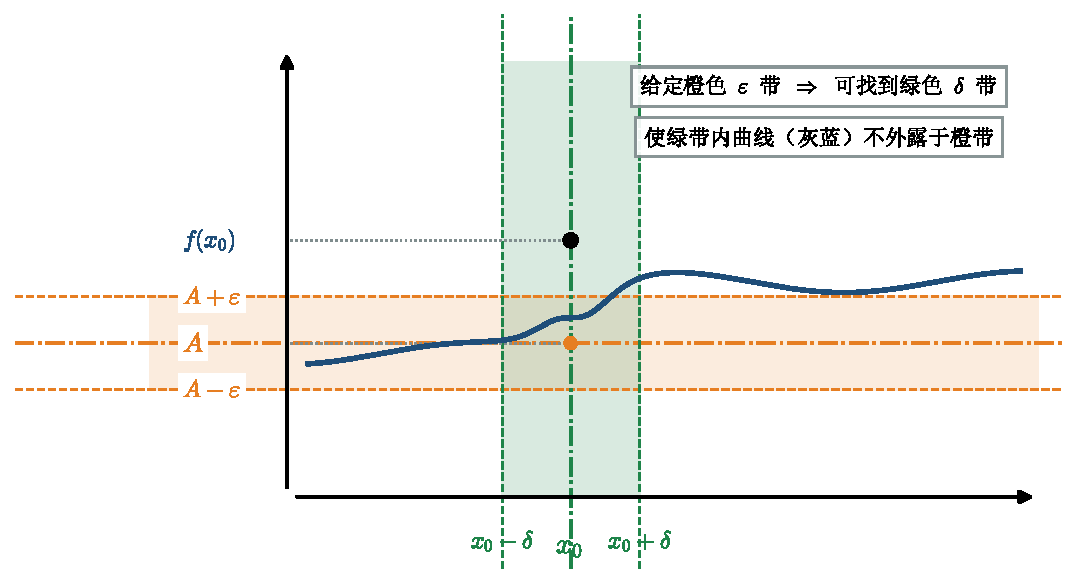
\includegraphics[width=0.94\textwidth]{figures/fig2_epsilon_delta.pdf}
  \caption{$\varepsilon$\text{-}$\delta$ 定义的“矩形控制”图像。给定水平橙色 $\eps$ 带（$A\pm\eps$），
           必须存在竖直绿色 $\delta$ 带（$x_0\pm\delta$），使得\emph{绿带内曲线不高出橙带}。
           注意 $x=x_0$ 处的值可以不看（去心），这正是“极限”与“连续”的差别。}
  \label{fig:epsdelta}
\end{figure}

\begin{keybox}[$\eps$-$\delta$ 与 $\eps$-$N$ 的对应]
\[
  \underbrace{\eps}_{\text{误差}}\ \longleftrightarrow\
  \underbrace{\delta}_{\text{控制 }x},\qquad
  \underbrace{n>N}_{\text{门槛}}\ \longleftrightarrow\
  \underbrace{0<\abs{x-x_0}<\delta}_{\text{门槛}} .
\]
唯一的实质差别是：$\eps$-$N$ 只需要“$n$ 足够大”，而 $\eps$-$\delta$ 需要“$x$ 足够\emph{接近}”，
因此 $x$ 可以\emph{从两侧}逼近，并且要排除 $x_0$ 本身。
\end{keybox}

\subsection{否定形式}

\begin{theorem}[函数极限不成立]\label{thm:neg-func}
“$\lim\limits_{x\to x_0}f(x)=A$” 不成立，当且仅当
\begin{equation}\label{eq:neg-epsdelta}
  \exists\eps_0>0,\quad \forall\delta>0,\quad \exists x:\ 0<\abs{x-x_0}<\delta
  \ \text{且}\ \abs{f(x)-A}\ge\eps_0 .
\end{equation}
\end{theorem}

\begin{proof}
与定理~\ref{thm:neg-seq} 同样的逐层取反。记
$P:\ \forall\eps\ \exists\delta\ \forall x\ \bigl(0<\abs{x-x_0}<\delta\Rightarrow\abs{f(x)-A}<\eps\bigr)$。
先把蕴含式改写：
\[
  \bigl(0<\abs{x-x_0}<\delta\Rightarrow\abs{f(x)-A}<\eps\bigr)
  \equiv
  \bigl(\abs{f(x)-A}\ge\eps\Rightarrow \neg(0<\abs{x-x_0}<\delta)\bigr),
\]
故其否定为
$\ \abs{f(x)-A}\ge\eps\ \wedge\ 0<\abs{x-x_0}<\delta$。于是
\[
  \overline P:\ \exists\eps>0\ \forall\delta>0\ \exists x\ 
  \bigl[\,0<\abs{x-x_0}<\delta\ \wedge\ \abs{f(x)-A}\ge\eps\,\bigr],
\]
即 \eqref{eq:neg-epsdelta}。

\end{proof}

\begin{figure}[H]
  \centering
  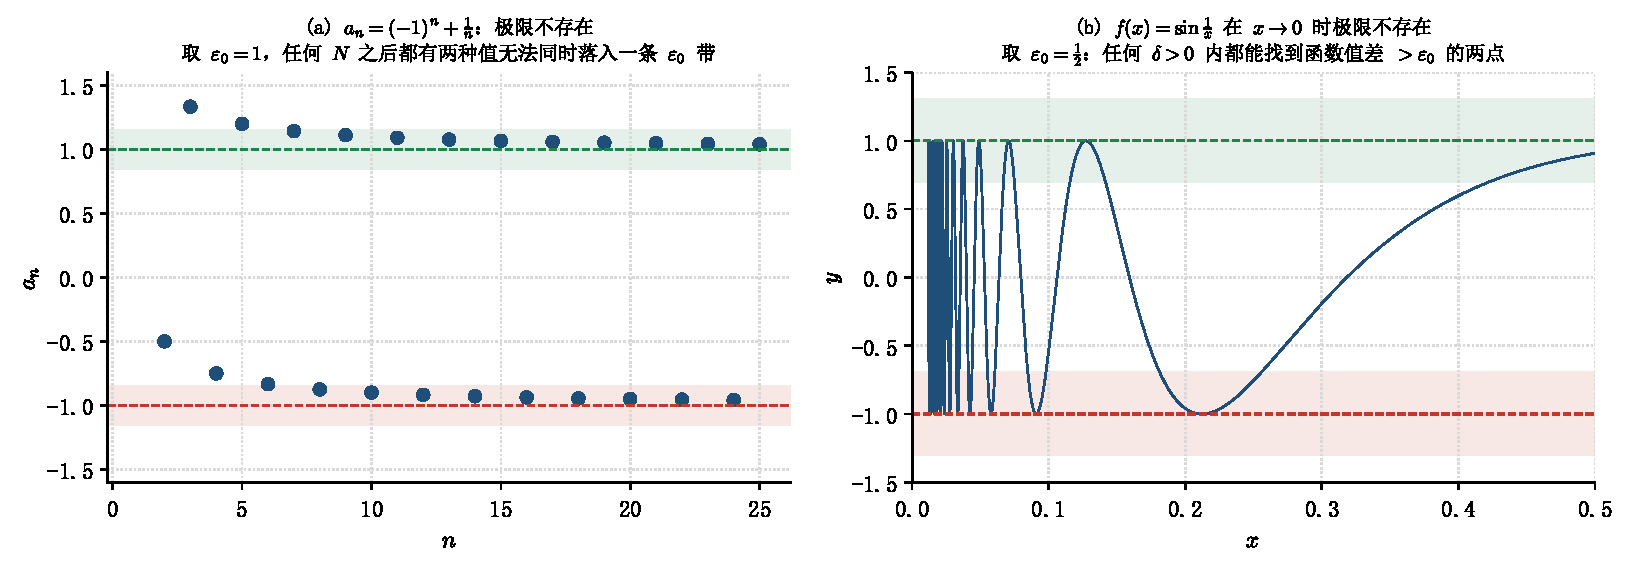
\includegraphics[width=0.99\textwidth]{figures/fig6_neg_limit.pdf}
  \caption{两个“极限不存在”的典型图像。(a) $a_n=(-1)^n+\frac1n$：取 $\eps_0=1$，
           无论 $N$ 多大，$N$ 之后总有落在 $+1$ 和 $-1$ 两处、彼此距离为 $2$ 的项。
           (b) $f(x)=\sin\frac1x$：取 $\eps_0=\frac12$，任何 $\delta>0$ 的邻域内都能找到两点，
           函数值差超过 $\eps_0$。}
  \label{fig:neglimit}
\end{figure}

\begin{counter}[$f(x)=\sin\frac1x$ 在 $x\to0$ 时极限不存在]
\end{counter}

\begin{proof}
取 $\eps_0=\frac12$（只要 $\eps_0<1$ 都可以）。对任意给定的 $\delta>0$，取
\[
  x_k=\frac{1}{2k\pi+\frac{\pi}{2}},\qquad y_k=\frac{1}{2k\pi-\frac{\pi}{2}} .
\]
当 $k$ 足够大时，$x_k,y_k\in(0,\delta)$，即 $0<x_k<\delta$、$0<y_k<\delta$。此时
\[
  f(x_k)=\sin(2k\pi+\tfrac{\pi}{2})=1,\qquad
  f(y_k)=\sin(2k\pi-\tfrac{\pi}{2})=-1 .
\]
若极限 $A$ 存在，则 $\abs{f(x_k)-A}<\eps_0$ 且 $\abs{f(y_k)-A}<\eps_0$，故
\[
  \abs{f(x_k)-f(y_k)}\le\abs{f(x_k)-A}+\abs{A-f(y_k)}<2\eps_0=1
  \quad\text{但实际 } \abs{f(x_k)-f(y_k)}=2>1,
\]
矛盾。因此极限不存在。这正好符合 \eqref{eq:neg-epsdelta}：
对任意 $\delta$，如上的 $x_k$ 就使 $\abs{f(x_k)-A}\ge\eps_0$。

\end{proof}

\subsection{单侧极限与无穷远处的极限}

\begin{definition}[单侧极限]
$\displaystyle\lim_{x\to x_0^+}f(x)=A$ 的定义是
\[
  \forall\eps>0\ \exists\delta>0\ \forall x:\ x_0<x<x_0+\delta\Rightarrow\abs{f(x)-A}<\eps .
\]
$\lim_{x\to x_0^-}$ 类似，只是把 $x_0<x<x_0+\delta$ 换成 $x_0-\delta<x<x_0$。
\end{definition}

\begin{theorem}\label{thm:two-sided}
$\lim\limits_{x\to x_0}f(x)=A\iff \lim\limits_{x\to x_0^+}f(x)=A=\lim\limits_{x\to x_0^-}f(x)$。
\end{theorem}

\begin{proof}
$(\Rightarrow)$ 设双侧极限为 $A$。给定 $\eps>0$，取定义~\ref{def:func-lim} 中的 $\delta$，
则当 $x_0<x<x_0+\delta$ 时自然满足 $0<\abs{x-x_0}<\delta$，故 $\abs{f(x)-A}<\eps$，
即右极限为 $A$；左极限同理。

$(\Leftarrow)$ 设双侧极限都是 $A$。给定 $\eps>0$，分别取 $\delta_1,\delta_2>0$ 使
\[
  x_0<x<x_0+\delta_1\Rightarrow\abs{f(x)-A}<\eps,\qquad
  x_0-\delta_2<x<x_0\Rightarrow\abs{f(x)-A}<\eps .
\]
取 $\delta=\min\{\delta_1,\delta_2\}$，则 $0<\abs{x-x_0}<\delta$ 时，$x$ 必落在左半或右半，
两种情形都有 $\abs{f(x)-A}<\eps$。

\end{proof}

\begin{definition}[无穷远极限，$\eps$-$M$ 语言]
$\displaystyle\lim_{x\to+\infty}f(x)=A$ 当且仅当
\[
  \forall\eps>0,\quad \exists M>0,\quad \forall x:\ x>M\Rightarrow\abs{f(x)-A}<\eps .
\]
$x\to-\infty$ 与 $x\to\infty$（即 $\abs x\to\infty$）分别把条件换成 $x<-M$ 与 $\abs x>M$。
\end{definition}

\begin{example}
用 $\eps$-$M$ 语言证明 $\displaystyle\lim_{x\to+\infty}\frac{1}{x}=0$。
\end{example}

\begin{proof}
给定 $\eps>0$，取 $M=\frac{1}{\eps}$。当 $x>M=\frac1\eps$ 时，
$\abs{\frac1x-0}=\frac1x<\frac{1}{M}=\eps$。故极限为 $0$。

\end{proof}

\subsection{极限的四则运算（$\eps$-$\delta$ 证明）}

\begin{theorem}[四则运算]\label{thm:arith}
设 $\lim\limits_{x\to x_0}f(x)=A$，$\lim\limits_{x\to x_0}g(x)=B$，则
\[
  \lim_{x\to x_0}\bigl(f\pm g\bigr)=A\pm B,\qquad
  \lim_{x\to x_0}\bigl(fg\bigr)=AB,\qquad
  \lim_{x\to x_0}\frac{f}{g}=\frac AB\ \ (B\neq0).
\]
\end{theorem}

\begin{proof}[证明（和与积，乘法是核心难点）]
\textbf{（一）和。}给定 $\eps>0$。取 $\delta_1,\delta_2>0$ 使
\[
  0<\abs{x-x_0}<\delta_1\Rightarrow\abs{f(x)-A}<\frac\eps2,\qquad
  0<\abs{x-x_0}<\delta_2\Rightarrow\abs{g(x)-B}<\frac\eps2 .
\]
取 $\delta=\min\{\delta_1,\delta_2\}$，则当 $0<\abs{x-x_0}<\delta$ 时
\[
  \abs{(f+g)(x)-(A+B)}\le\abs{f(x)-A}+\abs{g(x)-B}<\eps .
\]

\textbf{（二）积。}难点在于 $\abs{fg-AB}$ 不能直接用三角不等式拆成“误差 $\times$ 误差”
——那样得到的是 $\eps^2$ 量级，虽然也行，但更标准的做法是\textbf{插入中间项}：
\[
  fg-AB=\bigl(f-A\bigr)g+A\bigl(g-B\bigr),
\]
于是
\begin{equation}\label{eq:prod-bound}
  \abs{fg-AB}\le\abs{f-A}\cdot\abs{g}+\abs{A}\cdot\abs{g-B}.
\end{equation}
这里出现了 $\abs{g}$，必须事先\emph{控制住它}（这是乘法证明的关键技巧）。

\textbf{第 1 步：控制 $\abs g$ 与 $\abs f$ 的大小。}取 $\eps=1$（任取一个正数都行），
存在 $\delta_3>0$ 使 $0<\abs{x-x_0}<\delta_3$ 时 $\abs{g(x)-B}<1$，故
\[
  \abs{g(x)}\le\abs{g(x)-B}+\abs B<1+\abs B .
\]
同理存在 $\delta_4>0$ 使 $0<\abs{x-x_0}<\delta_4$ 时 $\abs{f(x)}<\abs A+1$
（这一步在证明 $\abs{f}$ 有界，供后面备用）。

\textbf{第 2 步：分配 $\eps$。}再取 $\delta_5,\delta_6>0$ 使
\[
  0<\abs{x-x_0}<\delta_5\Rightarrow\abs{f(x)-A}<\frac{\eps}{2(1+\abs B)},\qquad
  0<\abs{x-x_0}<\delta_6\Rightarrow\abs{g(x)-B}<\frac{\eps}{2(\abs A+1)} .
\]
（若 $A=0$，则取 $\abs A+1=1$ 即可，分母永远不为零——这是加 $1$ 的理由。）

\textbf{第 3 步：合并。}取 $\delta=\min\{\delta_3,\delta_5,\delta_6\}$。当 $0<\abs{x-x_0}<\delta$ 时，
把上述估计代入 \eqref{eq:prod-bound}：
\[
  \abs{f(x)g(x)-AB}
  \le\frac{\eps}{2(1+\abs B)}\cdot(1+\abs B)+\abs A\cdot\frac{\eps}{2(\abs A+1)}
  <\frac\eps2+\frac\eps2=\eps .
\]

\textbf{（三）商。}先证 $\lim\frac{1}{g}=\frac1B$。由 $B\neq0$，取 $\abs B/2$，
存在 $\delta_7>0$ 使 $0<\abs{x-x_0}<\delta_7$ 时 $\abs{g(x)-B}<\frac{\abs B}{2}$，于是
\[
  \abs{g(x)}\ge\abs B-\abs{g(x)-B}>\frac{\abs B}{2}>0,
\]
特别地 $g(x)\neq0$。此时
\[
  \abs{\frac{1}{g(x)}-\frac1B}=\frac{\abs{B-g(x)}}{\abs{g(x)}\abs B}
  \le\frac{2}{\abs B^{2}}\abs{g(x)-B} .
\]
给定 $\eps>0$，取 $\delta_8>0$ 使 $\abs{g(x)-B}<\frac{\abs B^{2}\eps}{2}$，合并即可。
最后用“积”的结论：$\frac fg=f\cdot\frac1g\to A\cdot\frac1B$。

\end{proof}

\begin{warnbox}[乘法证明最容易被扣分的地方]
\begin{itemize}
  \item \textbf{忘记先控制 $\abs g$}：直接写
        $\abs{fg-AB}\le\abs{f-A}\abs g+\abs A\abs{g-B}<\eps\abs g+\dots$ 是\emph{循环}的，
        因为 $\abs g$ 还依赖 $x$。
  \item \textbf{分母加了 $1$ 却解释不清}：$\frac{\eps}{2(\abs A+1)}$ 中的 $+1$ 是为了
        避免 $A=0$ 时除以零，也为了让界有统一的写法。
  \item \textbf{把 $\eps$ 当成固定数}：$\eps$ 是任给的；证明中可以用 $\eps/2$、$\eps/3$
        等，因为“$\eps/2$ 仍是任意的正数”。
\end{itemize}
\end{warnbox}

\subsection{Heine 定理（数列刻画）}

\begin{theorem}[Heine]\label{thm:heine}
设 $f$ 在 $\mathring\U(x_0,\eta)$ 上有定义。则
\[
  \lim_{x\to x_0}f(x)=A
  \iff
  \text{对\emph{任意}满足 } x_n\to x_0\ (x_n\neq x_0) \text{ 的数列，都有 } f(x_n)\to A .
\]
\end{theorem}

\begin{figure}[H]
  \centering
  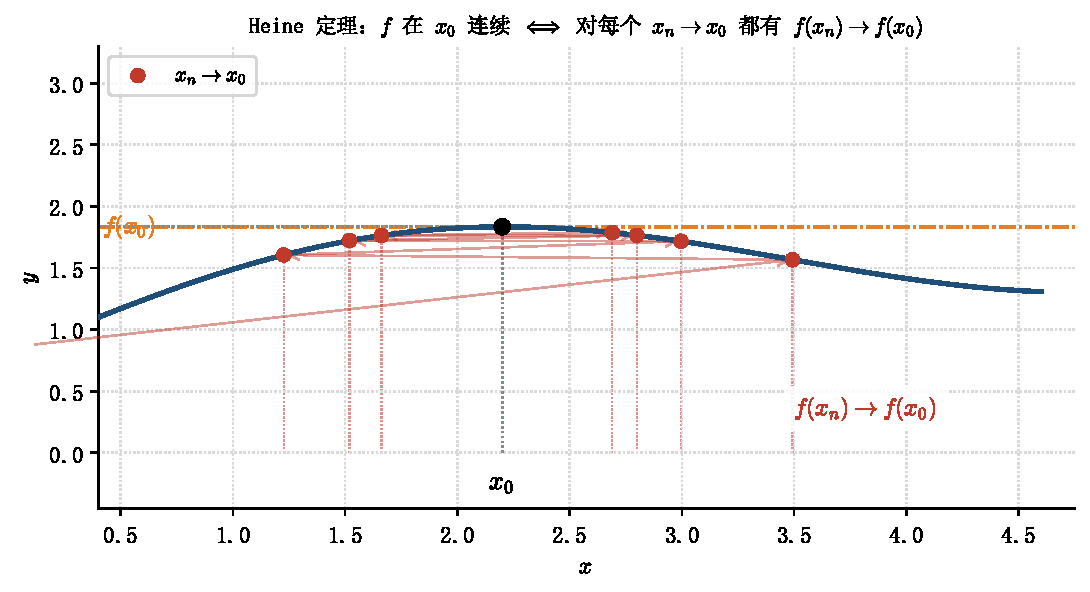
\includegraphics[width=0.92\textwidth]{figures/fig7_heine.pdf}
  \caption{Heine 定理的图像：若 $f$ 在 $x_0$ 连续，则任何收敛到 $x_0$ 的点列 $x_n$，
           其像 $f(x_n)$ 都被“吸”向 $f(x_0)$（图中红色箭头所示）。
           定理的\emph{逆向}用法（构造特殊数列来否定连续性）尤其重要。}
  \label{fig:heine}
\end{figure}

\begin{proof}[证明（$\Rightarrow$）]
设 $\lim_{x\to x_0}f(x)=A$，并设 $x_n\to x_0$、$x_n\neq x_0$。给定 $\eps>0$，
取 $\delta>0$ 使 $0<\abs{x-x_0}<\delta\Rightarrow\abs{f(x)-A}<\eps$。
由 $x_n\to x_0$ 且 $x_n\neq x_0$，存在 $N$ 使 $n>N$ 时 $0<\abs{x_n-x_0}<\delta$，
于是 $\abs{f(x_n)-A}<\eps$。故 $f(x_n)\to A$。

\end{proof}

\begin{proof}[证明（$\Leftarrow$，用反证法）]
设结论不成立，即 $\lim_{x\to x_0}f(x)\neq A$。由否定形式 \eqref{eq:neg-epsdelta}，
存在 $\eps_0>0$，使得\textbf{对每个} $\delta>0$ 都能找到 $x$ 满足
\[
  0<\abs{x-x_0}<\delta\ \text{且}\ \abs{f(x)-A}\ge\eps_0 .
\]
\textbf{构造}：对 $\delta=\frac1{n}$（$n=1,2,\dots$），取这样的 $x$ 记为 $x_n$，即
\[
  0<\abs{x_n-x_0}<\frac1n,\qquad \abs{f(x_n)-A}\ge\eps_0 .
\]
由第一式得 $x_n\neq x_0$ 且 $x_n\to x_0$；但由第二式，$f(x_n)$ 与 $A$ 的距离始终
$\ge\eps_0$，故 $f(x_n)\not\to A$。这与假设（任一 $x_n\to x_0$ 都有 $f(x_n)\to A$）矛盾。

这里用到了一条**选择公理**式的操作（对每个 $n$ 选一个 $x_n$），
在实分析中是标准做法：因为每个 $\delta$ 对应\emph{非空}的“坏点集”，故可逐次选取。

\end{proof}

\begin{corollary}[用数列否定极限]
$f(x)=\sin\frac1x$ 在 $x\to0$ 时无极限，也可以这样看：取
$x_n=\frac{1}{2n\pi+\pi/2}\to0$ 与 $y_n=\frac{1}{2n\pi-\pi/2}\to0$，
则 $f(x_n)\equiv1$、$f(y_n)\equiv-1$，两个像数列有不同的极限。由 Heine 定理，原极限不存在。
\end{corollary}

\newpage

% ============================ 第 3 章 ============================
\section{连续性：三种等价定义}

\subsection{定义与等价性}

\begin{definition}[点连续]\label{def:cont}
设 $f$ 在 $x_0$ 的某邻域内有定义。称 $f$ 在 $x_0$ \textbf{连续}，若
\begin{equation}\label{eq:cont}
  \forall\eps>0,\quad \exists\delta>0,\quad \forall x:\ \abs{x-x_0}<\delta
  \ \Rightarrow\ \abs{f(x)-f(x_0)}<\eps .
\end{equation}
\end{definition}

\begin{theorem}[三种等价的刻画]\label{thm:cont-equiv}
设 $f$ 在 $x_0$ 的某邻域内有定义。下列三条等价：
\begin{enumerate}[label=(\roman*)]
  \item $f$ 在 $x_0$ 连续（即 \eqref{eq:cont}）;
  \item $\lim\limits_{x\to x_0}f(x)=f(x_0)$;
  \item（Heine）对每个 $x_n\to x_0$（\emph{不}要求 $x_n\neq x_0$），都有 $f(x_n)\to f(x_0)$。
\end{enumerate}
\end{theorem}

\begin{proof}
\textbf{(i)$\Rightarrow$(ii)}：\eqref{eq:cont} 中的条件 $\abs{x-x_0}<\delta$
比极限定义中的 $0<\abs{x-x_0}<\delta$ 更宽（允许 $x=x_0$），所以 $\delta$ 可以直接沿用：
$x=x_0$ 时 $\abs{f(x_0)-f(x_0)}=0<\eps$ 自然成立。

\textbf{(ii)$\Rightarrow$(i)}：设 $\lim_{x\to x_0}f(x)=f(x_0)$。给定 $\eps>0$，
取 $\delta>0$ 使 $0<\abs{x-x_0}<\delta\Rightarrow\abs{f(x)-f(x_0)}<\eps$。
对 $x=x_0$ 的情形，$\abs{f(x_0)-f(x_0)}=0<\eps$ 也成立。合并两种情形即得 \eqref{eq:cont}。

\textbf{(ii)$\Leftrightarrow$(iii)}：由 Heine 定理~\ref{thm:heine}，
$\lim_{x\to x_0}f(x)=f(x_0)$ 等价于“任意 $x_n\to x_0$（$x_n\neq x_0$）有 $f(x_n)\to f(x_0)$”。
而 $x_n$ 列中若有\emph{无穷多}项等于 $x_0$，则这些项对应的 $f(x_n)=f(x_0)$，
不影响收敛性；把等于 $x_0$ 的项删去（或理解为恒等项）即化为 $x_n\neq x_0$ 的情形。
二者等价。

\end{proof}

\begin{example}[用 $\eps$-$\delta$ 证明具体函数的连续性]\label{ex:cont-x2}
证明 $f(x)=x^{2}$ 在任意 $x_0\in\R$ 连续。
\end{example}

\begin{proof}
\textbf{步骤 1（估计）}：核心是把 $\abs{x^2-x_0^2}$ 分解出 $\abs{x-x_0}$：
\[
  \abs{x^{2}-x_0^{2}}=\abs{x-x_0}\cdot\abs{x+x_0}
  \le\abs{x-x_0}\bigl(\abs{x-x_0}+2\abs{x_0}\bigr).
\]
\textbf{步骤 2（先限制 $\delta$）}：为了让括号里有界，预先要求 $\delta\le1$。
当 $\abs{x-x_0}<\delta\le1$ 时，$\abs{x+x_0}\le\abs{x-x_0}+2\abs{x_0}\le1+2\abs{x_0}$，于是
\[
  \abs{x^{2}-x_0^{2}}\le\abs{x-x_0}\bigl(1+2\abs{x_0}\bigr).
\]
\textbf{步骤 3（取 $\delta$）}：给定 $\eps>0$，取
\[
  \delta=\min\left\{1,\ \frac{\eps}{1+2\abs{x_0}}\right\}.
\]
\textbf{步骤 4（验证）}：$\abs{x-x_0}<\delta$ 时，
$\abs{x^2-x_0^2}<\delta\bigl(1+2\abs{x_0}\bigr)\le\eps$。

\end{proof}

\needspace{12\baselineskip}
\begin{tipbox}[“两步取 $\delta$” 模板]
含 $\abs{x+x_0}$、$\abs{x^2+1}$ 这类\emph{依赖 $x$} 的因子时，不能直接反解。标准做法是：
\begin{enumerate}[label=\arabic*., leftmargin=1.8em, topsep=2pt]
  \item 先无条件限制 $\delta\le1$（或别的常数），由此把因子换成只依赖 $x_0$ 的常数 $C(x_0)$；
  \item 再令 $\delta=\min\bigl\{1,\ \eps/C(x_0)\bigr\}$，取两者的 $\min$ 即可。
\end{enumerate}
这个模板适用于一切多项式、有理函数的连续性证明。
\end{tipbox}

\begin{example}[$f(x)=1/x$ 在 $x_0\neq0$ 处连续]\label{ex:cont-recip}
\end{example}

\begin{proof}
\textbf{步骤 1}：
\[
  \abs{\frac1x-\frac1{x_0}}=\frac{\abs{x_0-x}}{\abs{x}\,\abs{x_0}} .
\]
\textbf{步骤 2}：先取 $\delta\le\frac{\abs{x_0}}{2}$，则 $\abs{x}\ge\abs{x_0}-\abs{x-x_0}>\frac{\abs{x_0}}{2}$，
故 $\frac{1}{\abs x}<\frac{2}{\abs{x_0}}$，于是
\[
  \abs{\frac1x-\frac1{x_0}}\le\frac{2}{\abs{x_0}^{2}}\abs{x-x_0}.
\]
\textbf{步骤 3}：取 $\delta=\min\left\{\frac{\abs{x_0}}{2},\ \frac{\abs{x_0}^{2}\eps}{2}\right\}$，
\textbf{步骤 4}：则 $\abs{x-x_0}<\delta$ 时误差 $<\eps$。

\end{proof}

\begin{example}[Dirichlet 函数：处处不连续]\label{ex:dirichlet}
\[
  D(x)=\begin{cases}1,& x\in\Q,\\ 0,& x\notin\Q.\end{cases}
\]
证明 $D$ 在每一点都不连续。
\end{example}

\begin{proof}
固定任意 $x_0\in\R$。取 $\eps_0=\frac12$。对任意 $\delta>0$，
区间 $(x_0-\delta,x_0+\delta)$ 内既有有理数又有无理数（有理数与无理数都在 $\R$ 中稠密）。
\begin{itemize}
  \item 取有理数 $r\in(x_0-\delta,x_0+\delta)$：$D(r)=1$。
  \item 取无理数 $s\in(x_0-\delta,x_0+\delta)$：$D(s)=0$。
\end{itemize}
若 $D$ 在 $x_0$ 连续，则存在 $\delta$ 使邻域内所有 $x$ 满足 $\abs{D(x)-D(x_0)}<\frac12$。
不论 $D(x_0)$ 是 $0$ 还是 $1$，$D(r)$ 与 $D(s)$ 中必有一个与它相差 $1>\eps_0$，矛盾。
故 $D$ 处处不连续。

\end{proof}

\newpage

% ============================ 第 4 章 ============================
\section{一致连续：$\delta$ 能否与 $x_0$ 无关}

\subsection{定义}

\begin{definition}[一致连续]\label{def:unif}
设 $E\subseteq\R$，$f:E\to\R$。称 $f$ 在 $E$ 上\textbf{一致连续}，若
\begin{equation}\label{eq:unif}
  \forall\eps>0,\quad \exists\delta>0,\quad \forall x,y\in E:\ \abs{x-y}<\delta
  \ \Rightarrow\ \abs{f(x)-f(y)}<\eps .
\end{equation}
\end{definition}

\begin{keybox}[连续 vs 一致连续：只看量词顺序]
\[
  \begin{aligned}
    \text{连续（逐点）}:\quad& \forall x_0\in E\ \ \forall\eps>0\ \ \exists\delta>0\ \ \forall x:\ \abs{x-x_0}<\delta\Rightarrow\abs{f(x)-f(x_0)}<\eps\\
    \text{一致连续}:\quad& \forall\eps>0\ \ \exists\delta>0\ \ \forall x_0\in E\ \ \forall x:\ \abs{x-x_0}<\delta\Rightarrow\abs{f(x)-f(x_0)}<\eps
  \end{aligned}
\]
两者的差别只是\textbf{$\forall x_0$ 与 $\exists\delta$ 的先后}。
一致连续要求：$\delta$ \textbf{先于} $x_0$ 被选定，因而不能随 $x_0$ 变化。
换一种说法：一致连续的 $\delta=\delta(\eps)$，连续的 $\delta=\delta(\eps,x_0)$。
\end{keybox}

\begin{figure}[H]
  \centering
  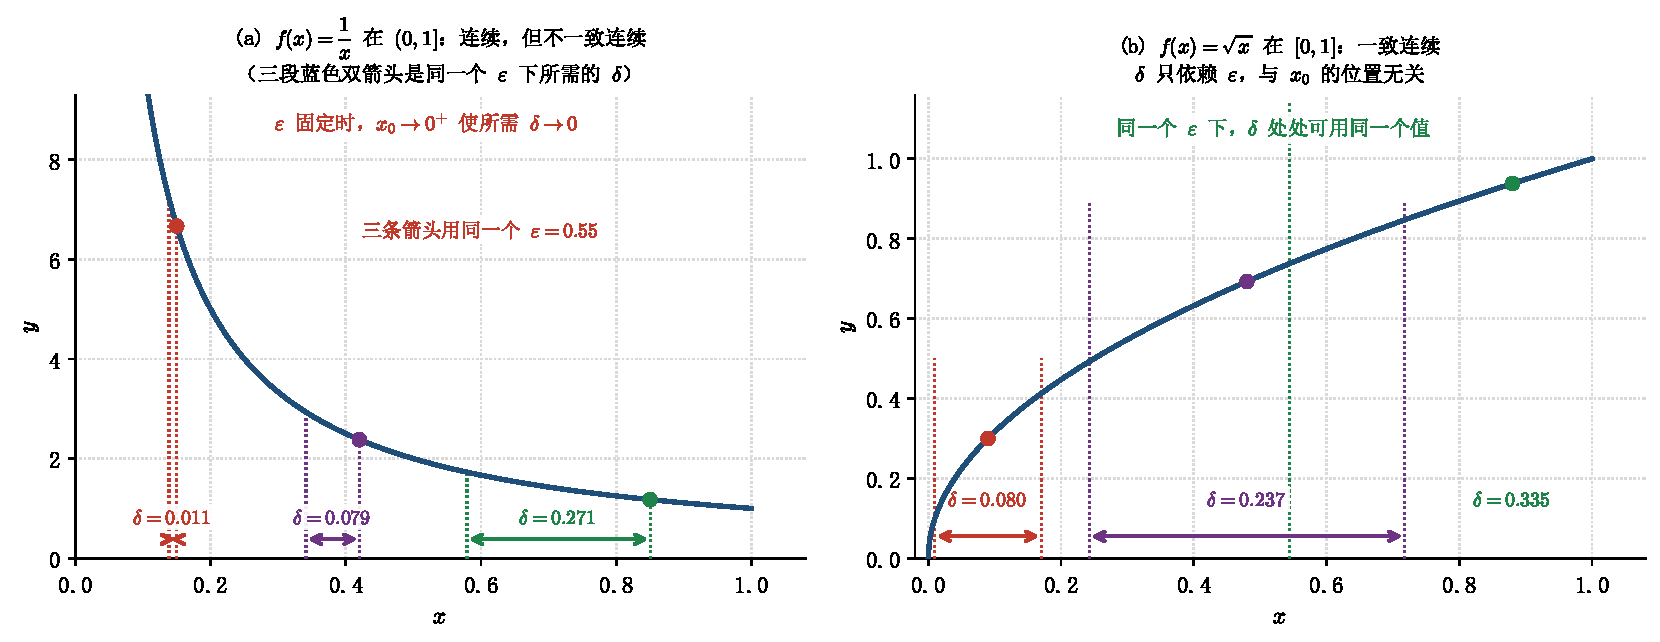
\includegraphics[width=0.99\textwidth]{figures/fig4_uniform.pdf}
  \caption{一致连续与否的对比。两图都固定同一个 $\eps$，用双箭头标出所需 $\delta$ 的\emph{长度}。
           (a) $f(x)=1/x$ 在 $(0,1]$：$x_0$ 越靠近 $0$，所需 $\delta$ 越小（$0.271\to0.079\to0.011$），
           无法统一，故非一致连续。(b) $f(x)=\sqrt x$ 在 $[0,1]$：各处所需的 $\delta$ 处在同一量级
           （$0.080$、$0.237$、$0.335$），存在统一下界，故一致连续。}
  \label{fig:uniform}
\end{figure}

\subsection{否定形式}

\begin{theorem}[非一致连续]\label{thm:neg-unif}
$f$ 在 $E$ 上\emph{不}一致连续，当且仅当
\begin{equation}\label{eq:neg-unif}
  \exists\eps_0>0,\quad \forall\delta>0,\quad \exists x,y\in E:\ 
  \abs{x-y}<\delta\ \text{且}\ \abs{f(x)-f(y)}\ge\eps_0 .
\end{equation}
\end{theorem}

\begin{proof}
逐层取反。命题 $P:\ \forall\eps\ \exists\delta\ \forall x\forall y\ \bigl(\abs{x-y}<\delta
\Rightarrow\abs{f(x)-f(y)}<\eps\bigr)$。同定理~\ref{thm:neg-func} 的推法，
蕴含式的否定为“前件成立且后件不成立”：
\[
  \overline P:\ 
  \exists\eps>0\ \forall\delta>0\ \exists x\exists y\ 
  \bigl[\abs{x-y}<\delta\ \wedge\ \abs{f(x)-f(y)}\ge\eps\bigr],
\]
即 \eqref{eq:neg-unif}。

\end{proof}

\begin{keybox}[实用判断法：找一对“坏点列”]
要证\emph{非}一致连续，只需构造两列 $x_n,y_n\in E$ 使
\[
  \abs{x_n-y_n}\to0\quad\text{但}\quad \abs{f(x_n)-f(y_n)}\ge\eps_0\ (\forall n).
\]
反过来，要证\emph{是}一致连续，就要对任意 $\eps$ 求出一个统一的 $\delta$。
\end{keybox}

\begin{example}[{$f(x)=1/x$ 在 $(0,1]$ 上非一致连续}]\label{ex:nonzero}
\end{example}

\begin{proof}
取 $x_n=\frac1n$，$y_n=\frac{1}{n+1}$，则
\[
  \abs{x_n-y_n}=\frac{1}{n(n+1)}\to0,
  \qquad
  \abs{f(x_n)-f(y_n)}=\abs{n-(n+1)}=1 .
\]
取 $\eps_0=1$。对任意 $\delta>0$，取 $n$ 足够大使 $\frac{1}{n(n+1)}<\delta$，
则这对点满足 \eqref{eq:neg-unif}。故 $f$ 在 $(0,1]$ 上非一致连续。

\textbf{注意}：$f(x)=1/x$ 在 $(0,1]$ 上\emph{每一点}都连续（例~\ref{ex:cont-recip}），
所以“连续”不能推出“一致连续”。根本原因是定义域 $(0,1]$ \emph{不是闭区间}。

\end{proof}

\begin{example}[{$f(x)=x^2$ 在 $[0,+\infty)$ 上非一致连续，但在 $[0,a]$ 上一致连续}]\label{ex:x2}
\end{example}

\begin{proof}
\textbf{(a) 在 $[0,\infty)$ 上非一致连续}：取 $x_n=n$，$y_n=n+\frac1n$，则
\[
  \abs{x_n-y_n}=\frac1n\to0,\qquad
  \abs{f(x_n)-f(y_n)}=\abs{n^{2}-(n+\tfrac1n)^{2}}
  =2+\frac{1}{n^{2}}\ \ge\ 2 .
\]
取 $\eps_0=2$，即符合 \eqref{eq:neg-unif}。

\textbf{(b) 在 $[0,a]$ 上一致连续}：
\[
  \abs{x^{2}-y^{2}}=\abs{x-y}\abs{x+y}\le\abs{x-y}\cdot 2a .
\]
给定 $\eps>0$，取 $\delta=\frac{\eps}{2a+1}$（加 $1$ 以处理 $a=0$），则 $\abs{x-y}<\delta$ 时
$\abs{x^2-y^2}<2a\cdot\frac{\eps}{2a+1}<\eps$。
\textbf{关键}：这里 $\delta$ 只依赖 $\eps$ 和 $a$，不依赖 $x_0$。

\end{proof}

\subsection{Cantor 定理：闭区间上连续即一致连续}

\begin{theorem}[Cantor, 一致连续性定理]\label{thm:cantor}
若 $f$ 在\emph{闭区间} $[a,b]$ 上连续，则 $f$ 在 $[a,b]$ 上一致连续。
\end{theorem}

\begin{proof}[证明（用有限覆盖定理）]
给定 $\eps>0$。

\textbf{第 1 步：每点给一个局部 $\delta$。}由 $f$ 在 $x_0$ 连续，存在 $\delta_{x_0}>0$ 使
\[
  \abs{x-x_0}<\delta_{x_0}\ \Rightarrow\ \abs{f(x)-f(x_0)}<\frac{\eps}{2} .
\]
于是只要 $x,y\in\bigl(x_0-\delta_{x_0},\,x_0+\delta_{x_0}\bigr)$，就有
\begin{equation}\label{eq:cantor-local}
  \abs{f(x)-f(y)}\le\abs{f(x)-f(x_0)}+\abs{f(x_0)-f(y)}<\eps .
\end{equation}

\textbf{第 2 步：形式化。}令 $\delta_{x_0}'=\frac{\delta_{x_0}}{2}$，
开区间族 $\bigl\{(x_0-\delta_{x_0}',\,x_0+\delta_{x_0}'):x_0\in[a,b]\bigr\}$ 覆盖 $[a,b]$。
由有限覆盖定理（Heine--Borel），存在有限个点 $x_1,\dots,x_m$ 使
\[
  [a,b]\subseteq\bigcup_{i=1}^{m}\bigl(x_i-\delta_{x_i}',\,x_i+\delta_{x_i}'\bigr).
\]

\textbf{第 3 步：取统一 $\delta$。}令
\[
  \delta=\min_{1\le i\le m}\delta_{x_i}'=\frac12\min_{1\le i\le m}\delta_{x_i}>0 .
\]
（有限多个正数的最小值仍为正——这正是“有限”覆盖不可省的原因；无限族的 $\inf$ 可能为 $0$。）

\textbf{第 4 步：验证。}设 $x,y\in[a,b]$ 且 $\abs{x-y}<\delta$。
由覆盖，$x\in(x_i-\delta_{x_i}',x_i+\delta_{x_i}')$ 对某个 $i$ 成立。于是
\[
  \abs{y-x_i}\le\abs{y-x}+\abs{x-x_i}<\delta+\delta_{x_i}'
  \le\delta_{x_i}'+\delta_{x_i}'=\delta_{x_i} .
\]
且同样 $\abs{x-x_i}<\delta_{x_i}'<\delta_{x_i}$。故 $x,y$ 都落在 $(x_i-\delta_{x_i},x_i+\delta_{x_i})$ 内，
由 \eqref{eq:cantor-local} 得 $\abs{f(x)-f(y)}<\eps$。
而 $\delta$ 只依赖 $\eps$（通过有限个 $\delta_{x_i}$），与 $x,y$ 无关。

\end{proof}

\begin{example}[{$\sqrt x$ 在 $[0,1]$ 上一致连续 —— 直接验证}]\label{ex:sqrt-unif}
\end{example}

\begin{proof}
用恒等式 $(\sqrt x-\sqrt y)(\sqrt x+\sqrt y)=x-y$。不妨设 $x\ge y\ge0$，则 $\sqrt x+\sqrt y\ge\sqrt x-\sqrt y$，故
\[
  \abs{\sqrt x-\sqrt y}=\frac{\abs{x-y}}{\sqrt x+\sqrt y}
  \le\frac{\abs{x-y}}{\sqrt x-\sqrt y}.
\]
若 $x\neq y$，两边乘以 $\sqrt x-\sqrt y>0$ 得 $\abs{\sqrt x-\sqrt y}^{2}\le\abs{x-y}$，即
\[
  \abs{\sqrt x-\sqrt y}\le\sqrt{\abs{x-y}} .
\]
给定 $\eps>0$，取 $\delta=\eps^{2}$。则 $\abs{x-y}<\delta$ 时 $\abs{\sqrt x-\sqrt y}<\eps$。
$\delta$ 与 $x,y$ 无关，故一致连续。

\textbf{注意}：这里 $\delta=\eps^{2}$ 与位置无关，但 $\delta\to0$ 的速度是 $\eps^{2}$ 级的，
比线性型（如例~\ref{ex:x2}(b)）慢——这正说明 $\sqrt x$ 在 $0$ 处“导数无穷大”，
却仍可以是（Hölder）一致连续的。

\end{proof}

\begin{theorem}[一致连续的基本性质]\label{thm:unif-prop}
\begin{enumerate}[label=(\roman*)]
  \item 若 $f$ 在 $E$ 上一致连续，则 $f$ 在 $E$ 上连续；
  \item 若 $f$ 在 $E$ 上一致连续，则 $f$ 把 Cauchy 列映为 Cauchy 列
        （称为 \textbf{Cauchy 连续}）；
  \item 若 $E$ 有界且 $f$ 在 $E$ 上一致连续，则 $f$ 在 $E$ 上有界。
\end{enumerate}
（(i) 的逆不成立，见例~\ref{ex:nonzero}。）
\end{theorem}

\begin{proof}
\textbf{(i)}：一致连续的 $\delta$ 对每个 $x_0$ 都适用，当然满足逐点连续的要求
（取同一个 $\delta$ 即可）。

\textbf{(ii)}：设 $\{x_n\}\subseteq E$ 是 Cauchy 列，给定 $\eps>0$。
由一致连续取 $\delta>0$ 使 $\abs{x-y}<\delta\Rightarrow\abs{f(x)-f(y)}<\eps$。
由 Cauchy 性取 $N$ 使 $m,n>N$ 时 $\abs{x_m-x_n}<\delta$，于是 $\abs{f(x_m)-f(x_n)}<\eps$。
故 $\{f(x_n)\}$ 是 Cauchy 列。

\textbf{(iii)}：取 $\eps=1$，得 $\delta>0$ 使 $\abs{x-y}<\delta\Rightarrow\abs{f(x)-f(y)}<1$。
把有界区间 $E$（设 $E\subseteq[-K,K]$）分成有限段
$I_j=[-K+(j-1)\frac\delta2,\,-K+j\frac\delta2]$，共 $m=\lceil\frac{4K}{\delta}\rceil$ 段，
每段长度 $\frac\delta2<\delta$。每段取一点 $\xi_j\in I_j\cap E$（若非空），
则对 $x\in I_j\cap E$，$\abs{x-\xi_j}<\delta$，故
$\abs{f(x)}\le\abs{f(x)-f(\xi_j)}+\abs{f(\xi_j)}<1+\abs{f(\xi_j)}$。
取 $M=\max_j\bigl(1+\abs{f(\xi_j)}\bigr)$（有限个），则 $\abs{f(x)}\le M$ 对一切 $x\in E$ 成立。

\end{proof}

\subsection{三种反例：把“连续”与“一致连续”彻底分开}

\begin{figure}[H]
  \centering
  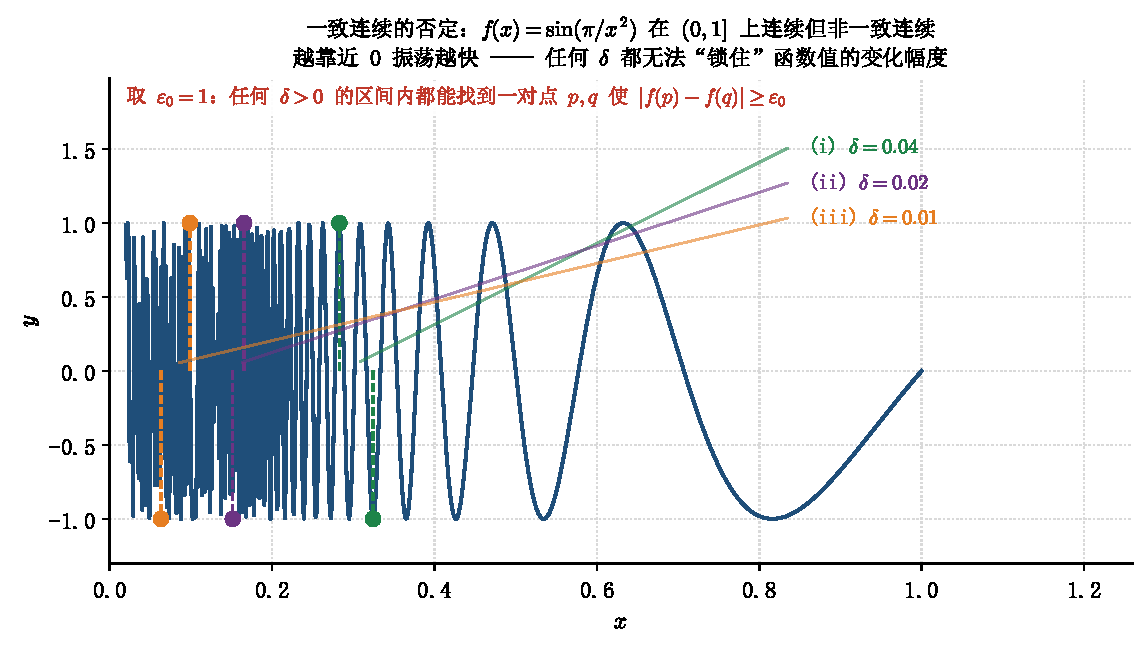
\includegraphics[width=0.93\textwidth]{figures/fig5_uniform_neg.pdf}
  \caption{$f(x)=\sin(\pi/x^2)$ 在 $(0,1]$ 上连续但非一致连续。
           取 $\eps_0=1$：即使把 $\delta$ 压到 $0.01$（(iii)），区间内仍有两点 $p,q$ 使
           $\abs{f(p)-f(q)}\ge\eps_0$。越靠近 $0$，振荡频率越高——这是“紧性失效”的直观原因。}
  \label{fig:unifneg}
\end{figure}

\begin{counter}[{$f(x)=\sin(x^{2})$ 在 $[0,\infty)$ 上非一致连续}]
虽然它在每点连续，且 $\abs f\le1$（有界），但仍非一致连续。
\end{counter}

\begin{proof}
取
\[
  x_n=\sqrt{2n\pi+\frac{\pi}{2}},\qquad y_n=\sqrt{2n\pi-\frac{\pi}{2}} .
\]
则 $\sin x_n^{2}=1$，$\sin y_n^{2}=-1$，故 $\abs{f(x_n)-f(y_n)}=2$。而
\[
  \abs{x_n-y_n}=\frac{\abs{x_n^{2}-y_n^{2}}}{x_n+y_n}=\frac{\pi}{x_n+y_n}\ \longrightarrow\ 0
\]
（因为 $x_n,y_n\to\infty$）。取 $\eps_0=2$，即符合定理~\ref{thm:neg-unif}。

\end{proof}

\begin{keybox}[小结：连续 $\Rightarrow$ 一致连续 需要什么？]
\begin{center}
\begin{tabular}{@{}llll@{}}
\toprule
\textbf{定义域} & \textbf{连续} & \textbf{一致连续} & \textbf{说明}\\
\midrule
闭区间 $[a,b]$ & 有 & \textbf{必有}（Cantor 定理） & 紧性\\
开区间 $(0,1]$ & 有 & 未必（$1/x$） & 非紧\\
$[0,\infty)$ & 有 & 未必（$x^2$、$\sin x^2$） & 无界\\
$\R$ 上有界连续 & 有 & 未必（$\sin x^2$） & 有界不够\\
闭区间 + 连续 & 有 & 有 & 定理~\ref{thm:cantor}\\
\bottomrule
\end{tabular}
\end{center}
一句话：\textbf{“紧集上的连续函数自动一致连续”；一切反例都源于定义域不紧或函数不有界。}
\end{keybox}

\newpage

% ============================ 第 5 章 ============================
\section{常见错误与陷阱}

本节把初学者最常犯的错误集中起来，每条都给出\textbf{错在哪}与\textbf{正确写法}。

\subsection{量词顺序错误}

\begin{warnbox}[错误 1：把 $\forall\eps\exists N$ 写成 $\exists N\forall\eps$]
\textbf{错误写法}：“对每个数列，存在 $N$ 使对任意 $\eps>0$ 有 $\abs{a_n-A}<\eps$。”
\par\smallskip
\textbf{诊断}：取 $a_n=A+\frac1n$，则 $\abs{a_n-A}=\frac1n>0$ 对一切 $n$ 成立，
不存在这样的 $N$。该写法实际上要求\emph{从某项起 $a_n$ 恒等于 $A$}，这比收敛强得多。
\par\smallskip
\textbf{正确写法}：$\forall\eps>0\ \exists N\ \forall n>N:\abs{a_n-A}<\eps$。
$N$ 是 $\eps$ 的\emph{函数}，$\eps$ 越小 $N$ 越大，这是允许的。
\end{warnbox}

\begin{warnbox}[错误 2：在一致连续里让 $\delta$ 依赖 $x_0$]
\textbf{错误写法}（证明 $f$ 一致连续时）：“取 $\delta=\delta(\eps,x_0)$……”
\par\smallskip
\textbf{诊断}：这就退化为逐点连续了。一致连续的整个内容就在于\textbf{$\delta$ 不能带 $x_0$}。
\par\smallskip
\textbf{正确写法}：先固定 $\eps$，然后指出对所有 $x_0$ 都能用同一个 $\delta$。
含 $\abs{x-x_0}$ 的项的界要化成只依赖 $\eps$（必要时借助定义域紧性）。
\end{warnbox}

\subsection{把等式与不等式混用}

\begin{warnbox}[错误 3：证明等式时用“$\le$”糊弄过去]
\textbf{错误写法}：欲证 $f$ 在 $x_0$ 连续，写
“$\abs{f(x)-f(x_0)}\le \abs{x-x_0}\to0$，所以连续。”
\par\smallskip
\textbf{诊断}：思路正确，但这只是“提示”，不是 $\eps$-$\delta$ 证明；
而且如果中间放缩的系数依赖 $x$，结论不成立。
\par\smallskip
\textbf{正确写法}：把系数化成只依赖 $x_0$ 的常数（例~\ref{ex:cont-x2} 的“两步取 $\delta$”），
再显式给出 $\delta=\min\{\dots\}$。
\end{warnbox}

\begin{warnbox}[错误 4：取 $\eps$ 时用了 $x$]
\textbf{错误写法}：“令 $\eps=\abs{x-x_0}$，则 $\abs{f(x)-f(x_0)}<\abs{x-x_0}$。”
\par\smallskip
\textbf{诊断}：$\eps$ 必须\emph{事先}给定、与 $x$ 无关。用它来控制 $x$ 是本末倒置。
\par\smallskip
\textbf{正确写法}：$\eps$ 是外部给的常数，$\delta$ 由它确定。
\end{warnbox}

\subsection{关于 cauchy 准则的误解}

\begin{warnbox}[错误 5：以为 Cauchy 准则在任何数域都成立]
\textbf{诊断}：Cauchy 准则的充分性等价于\emph{完备性}。
在 $\Q$ 上取 $a_n=$ $\sqrt2$ 的 $n$ 位截断小数，它满足 \eqref{eq:cauchy} 但极限 $\sqrt2\notin\Q$。
\par\smallskip
\textbf{正确写法}：在 $\R$（或任何 Banach 空间）中成立；在 $\Q$ 上需要对序列额外要求或换用完备化。
\end{warnbox}

\begin{warnbox}[错误 6：忽略“$x\neq x_0$”]
\textbf{错误写法}：把函数极限定义写成 $\abs{x-x_0}<\delta\Rightarrow\dots$（丢掉 $0<$）。
\par\smallskip
\textbf{诊断}：这样得到的其实是\emph{连续}（并要求 $f(x_0)=A$），
而 $f(x)=\frac{\sin x}{x}$ 在 $x_0=0$ 处根本没有定义，该写法会判定极限不存在。
\par\smallskip
\textbf{正确写法}：极限定义中保留 $0<\abs{x-x_0}<\delta$；
连续定义则用 $\abs{x-x_0}<\delta$ 并比较 $f(x_0)$。
\end{warnbox}

\newpage

% ============================ 附录 ============================
\appendix
\section*{附录 A\quad 定义与否定形式速查}
\addcontentsline{toc}{section}{附录 A\quad 定义与否定形式速查}

{\small
\renewcommand{\arraystretch}{1.75}
\begin{table}[H]
\centering
\begin{tabular}{@{}p{0.19\linewidth}p{0.36\linewidth}p{0.36\linewidth}@{}}
\toprule
\textbf{命题} & \textbf{肯定形式} & \textbf{否定形式} \\
\midrule
$a_n\to A$
 & $\forall\eps>0\ \exists N\ \forall n>N:\abs{a_n-A}<\eps$
 & $\exists\eps_0>0\ \forall N\ \exists n>N:\abs{a_n-A}\ge\eps_0$ \\
$\{a_n\}$ Cauchy
 & $\forall\eps>0\ \exists N\ \forall m,n>N:\abs{a_m-a_n}<\eps$
 & $\exists\eps_0>0\ \forall N\ \exists m,n>N:\abs{a_m-a_n}\ge\eps_0$ \\
$\lim\limits_{x\to x_0}f=A$
 & $\forall\eps>0\ \exists\delta>0\ \forall x:0<\abs{x-x_0}<\delta\Rightarrow\abs{f-A}<\eps$
 & $\exists\eps_0>0\ \forall\delta>0\ \exists x:0<\abs{x-x_0}<\delta\wedge\abs{f-A}\ge\eps_0$ \\
$f$ 在 $x_0$ 连续
 & $\forall\eps>0\ \exists\delta>0\ \forall x:\abs{x-x_0}<\delta\Rightarrow\abs{f(x)-f(x_0)}<\eps$
 & $\exists\eps_0>0\ \forall\delta>0\ \exists x:\abs{x-x_0}<\delta\wedge\abs{f(x)-f(x_0)}\ge\eps_0$ \\
$f$ 在 $E$ 一致连续
 & $\forall\eps>0\ \exists\delta>0\ \forall x,y\in E:\abs{x-y}<\delta\Rightarrow\abs{f(x)-f(y)}<\eps$
 & $\exists\eps_0>0\ \forall\delta>0\ \exists x,y\in E:\abs{x-y}<\delta\wedge\abs{f(x)-f(y)}\ge\eps_0$ \\
$\lim\limits_{x\to\infty}f=A$
 & $\forall\eps>0\ \exists M>0\ \forall x:\abs x>M\Rightarrow\abs{f-A}<\eps$
 & $\exists\eps_0>0\ \forall M>0\ \exists x:\abs x>M\wedge\abs{f-A}\ge\eps_0$ \\
\bottomrule
\end{tabular}
\end{table}
}

\section*{附录 B\quad 证明模板清单}
\addcontentsline{toc}{section}{附录 B\quad 证明模板清单}

\begin{keybox}[模板 1：$\eps$-$N$ / $\eps$-$\delta$ 直接验证]
\textbf{放缩 $\to$ 反解 $\to$ 取 $N$ 或 $\delta$ $\to$ 回代。}
适用于：具体数列/具体函数的极限，能显式解出不等式。
\end{keybox}

\begin{keybox}[模板 2：两步取 $\delta$]
\textbf{先无条件限制 $\delta\le 1$（或 $\abs{x-x_0}\le\frac{\abs{x_0}}{2}$）以控制变系数，
再令 $\delta=\min\{\text{限制值},\ \eps/\text{常数}\}$。}
适用于：多项式、有理函数、$\abs{x}$ 出现在分母或系数中的情形。
\end{keybox}

\begin{keybox}[模板 3：$\eps/2$ 分配]
\textbf{把 $\eps$ 拆成 $\eps/2+\eps/2$ 分给两项；若要 $k$ 项就拆成 $k$ 份。}
适用于：三角不等式求和、（有限）个误差项叠加。
\end{keybox}

\begin{keybox}[模板 4：先控制因子大小，再分配 $\eps$]
\textbf{先用某个固定 $\eps_1$（如 $1$）得到 $\abs{g(x)}\le M$，再用 $\eps/(2M)$ 控制误差。}
适用于：乘积、商的极限（定理~\ref{thm:arith}）。
\end{keybox}

\begin{keybox}[模板 5：反证 $+$ 构造坏点列]
\textbf{否定形式 $\to$ 对每个 $\delta=1/n$ 取坏点 $\to$ 得到矛盾。}
适用于：证明“极限不存在”“不一致连续”以及 Heine 定理的逆向。
\end{keybox}

\vfill
\begin{center}
{\color{mainc}\rule{0.4\linewidth}{0.8pt}}\\[6pt]
{\kaishu\small $\varepsilon$ 是挑战，$\delta$ 是应答。\\[2pt]
数学分析中几乎所有“存在性”证明，都是\textbf{先固定一个量，再为它配一个量}。\\[2pt]
看懂量词的顺序，就看懂了整个分析。}
\end{center}

\end{document}
